%%Por lo que si se considera el estado inicial del Universo aleatorio, bajo ciertas consideraciones, entonces, los postulados sobre las inhomogeneidades en el Universo necesitan ser estadísticas por naturaleza. 

El modelo inflacionario cosmológico establece las condiciones iniciales del Universo y su evolución. En la actualidad, la evidencia experimental utilizada para válidar el modelo reside en la medición de la radiación del fondo cósmico de microondas \CMB~(\textbf{C}osmic \textbf{M}icrowave \textbf{B}ackground), medido en los años 1960, y el corrimiento al rojo de la radiación electromagnética. % Se teoriza que unos 379 000 años después del Big Bang (per\'iodo de la última dispersión) la temperatura del Universo era de unos $3000~K$, la misma ha caído en un factor de aproximadamente $1100~K$ debido a la expansión del Universo. 
%Según se expande el Universo, los fotones del \CMB ~ se desplazan hacia el rojo, haciendo que la temperatura de radiación sea inversamente proporcional al factor de escala del Universo.

La radiación~\CMB~parece a primera vista isótropa, pero posee pequeñas anisotropías en la temperatura las cuales son producto de la distribución de la materia del universo. Estas inhomogeneidades fueron detectadas por el satélite de la NASA \textbf{COBE} (\textbf{C}osmic \textbf{B}ackground \textbf{E}xplorer) entre 1989 y 1996. 
En el 2001 NASA lanza el~\WMAP~(\textbf{W}ilkinson \textbf{M}icrowave \textbf{A}nisotropy \textbf{P}robe), %\footnote{Página de origen: \url{https://wmap.gsfc.nasa.gov/media/121238/index.html}} satélite capaz de estudiar con gran detalle la radiación~\CMB, . 
 este estudió con mayor resolución angular las anisotropías del \CMB, revelan un universo en expansión formado en un 4\% de materia bariónica y 22 \% de materia oscura. 
El 2009 la Agencia Espacial Europea lanzó la sonda Planck \citep{planck_collaboration_planck_2019}, como satélite de capacidades mucho mayores a sus predecesores, con una resolución y sensibilidad mejoradas. Debido a la alta precisión del mapa de Planck se revela algunas características peculiares hasta el momento inexplicables que pueden requerir una nueva física.

% ems: Citar párrafo anterior. Te sugiero los artículos originales de las colaboraciones.

\begin{figure}[!t]
    \centering
    %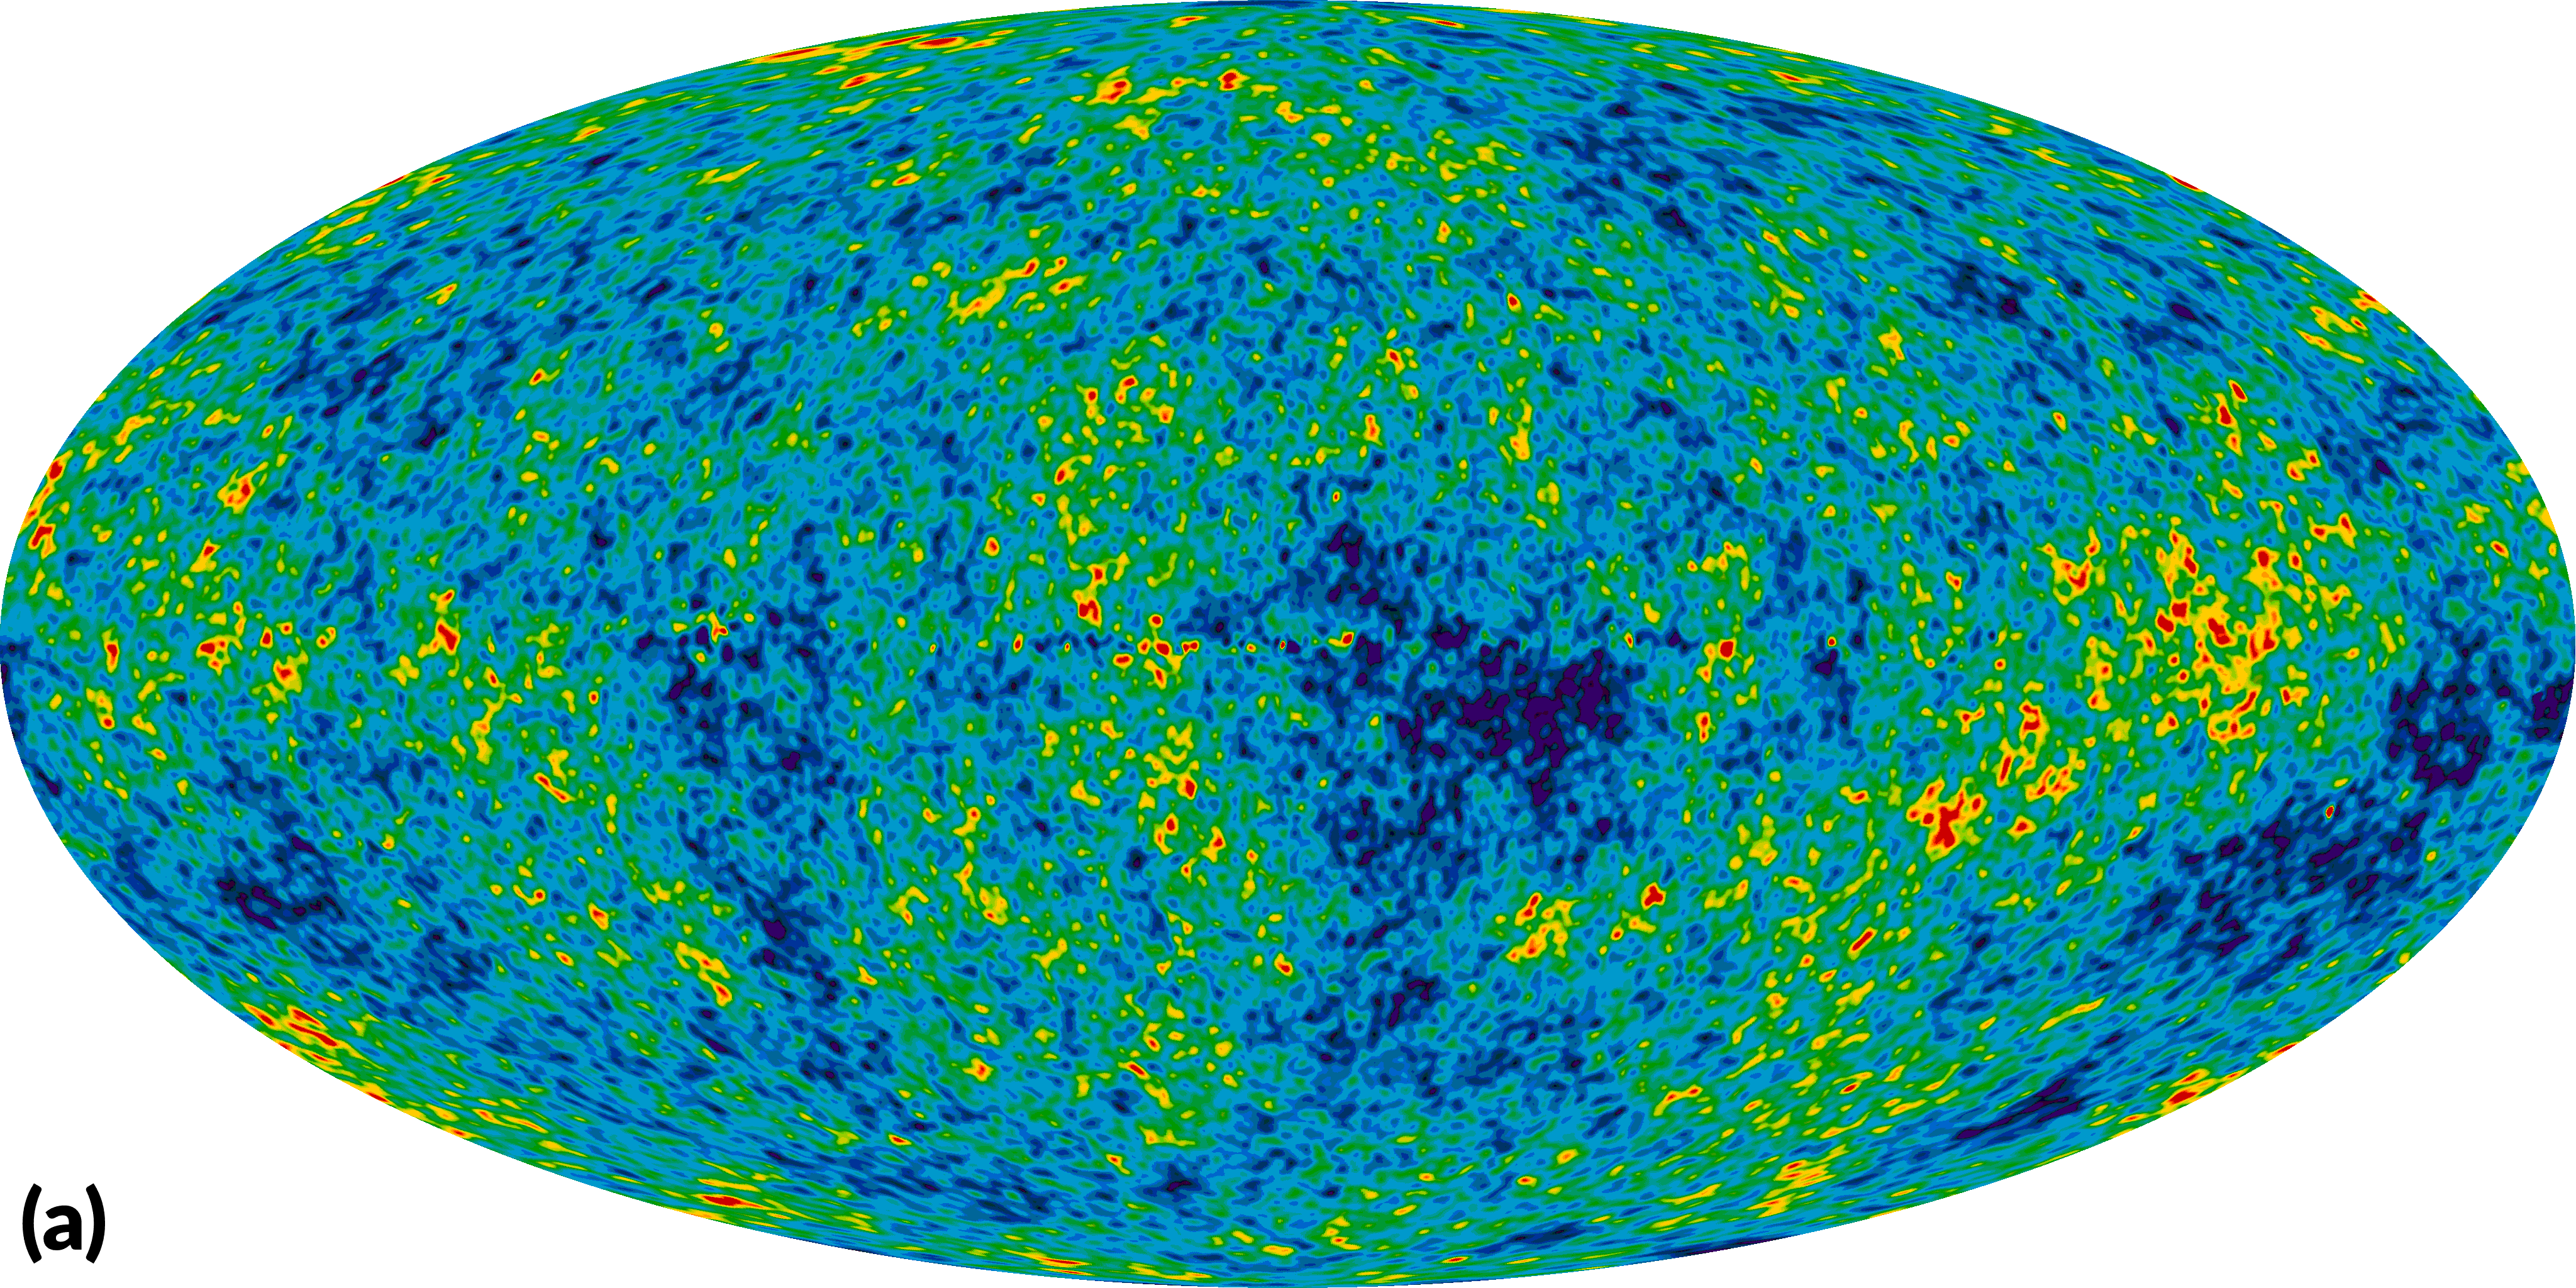
\includegraphics[width=0.49\textwidth]{Fisica_de_Particulas/imagenes/universo.png}
    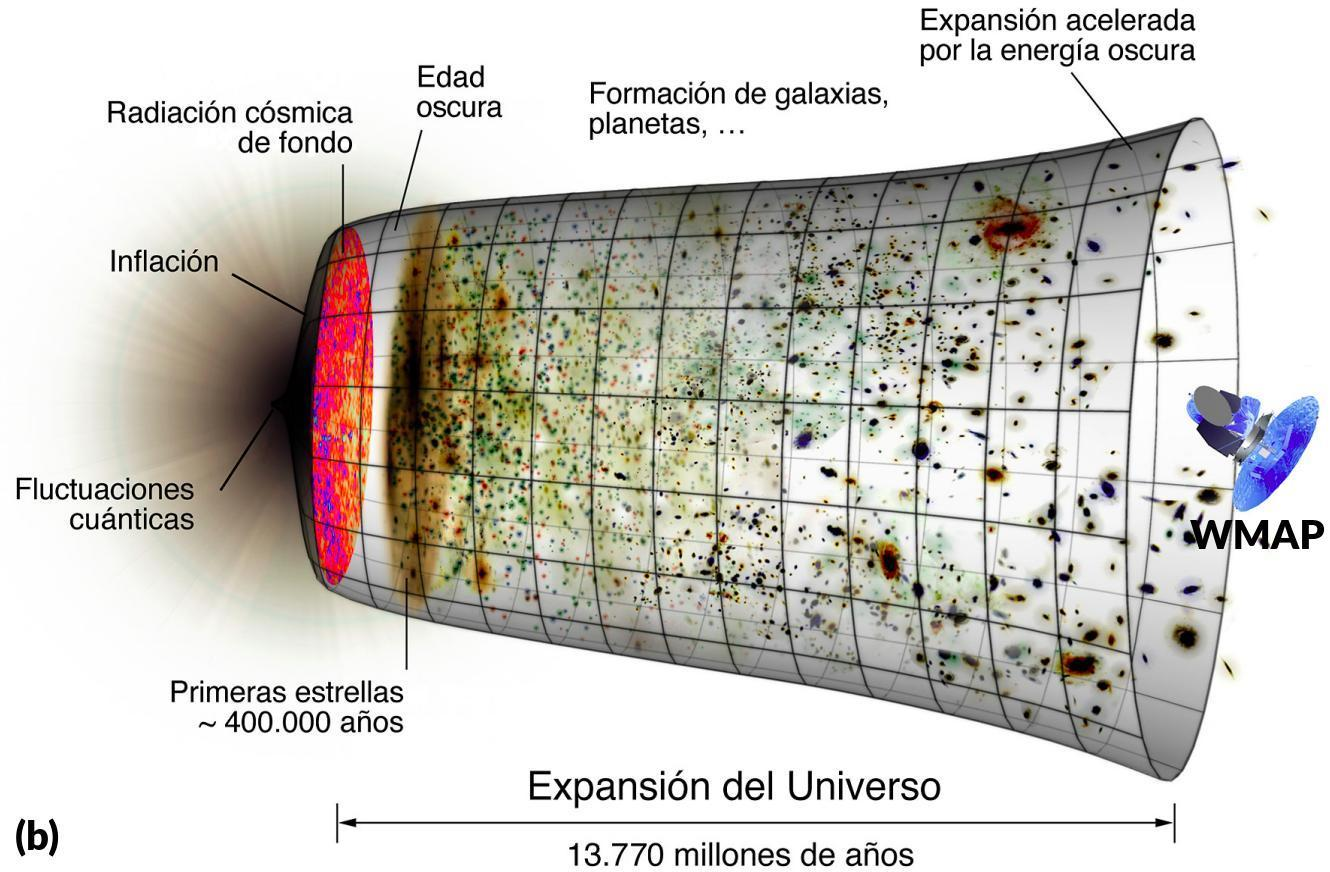
\includegraphics[width=0.49\textwidth]{Fisica_de_Particulas/imagenes/Universo_evo0.jpg}
    \caption[Representación de la evolución del universo]{Representación de la evolución del universo a lo largo de 13.77 mil millones de a\~nos. \footnotemark
    %\url{https://wmap.gsfc.nasa.gov/media/060915/index.html}
    %(a) Mapa de anisotropías de temperatura de~\CMB~según lo observado por el telescopio ~\WMAP. %Página de origen: \url{https://wmap.gsfc.nasa.gov/media/121238/index.html
    }
    \label{universo}
\end{figure}
\footnotetext{Página de origen: \url{https://wmap.gsfc.nasa.gov/media/060915/index.html}}

Entre los hallazgos más importantes están:
\begin{itemize}
\item Las fluctuaciones en las temperaturas de \CMB ~ a grandes escalas angulares no coinciden con las predichas por el \ME. %; sus señales no son tan fuertes como se esperaba de la estructura a menor escala revelada por Planck.
\item Confirma la asimetría en las temperaturas medias en hemisferios opuestos del cielo. Esto contradice el principio cosmológico que estipula la isotropía del universo.
\item Confirma la existencia de una región fría extendida sobre un parche de cielo.
\end{itemize}

Esto permitió obtener valores mas refinados de los obtenidos por el ~ \WMAP ~ de la composición de la materia que compone el universo, sus resultados fueros 4.9\% de la masa bariónica. La materia oscura, que hasta ahora solo se ha detectado indirectamente por su influencia gravitacional, representa el 26.8\% y la energía oscura con un porciento de 68.3\% siento la fuerza misteriosa posible responsable de acelerar la expansión del Universo.

Los datos de Planck establecen la velocidad a la que el Universo se está expandiendo hoy(constante de Hubble) con $H_0 = 67.15~km~s^{-1} ~Mpc^{-1}$ implicando que la edad del Universo teorizada en la Fig. \ref{universo}b. 

%Según el Principio cosmológico debemos pensar que cualquier punto del universo es un buen punto para ser considerado como un supuesto ``centro'', pues desde cualquier punto tendremos las mismas observaciones en cuanto a expansión del universo y densidad, esta idea es necesaria para obtener el valor de la densidad crítica ($\rho_c$) que es la densidad de la materia en el universo necesaria para detener la expansión del mismo en un tiempo infinito, con valor de $\rho_c = 1.88~h 2 \times 10−26 kg/m^3$ implementando \href{https://es.wikipedia.org/wiki/Ecuaciones_de_Friedmann}{las ecuaciones de Friedmann} (ver referencia \cite{vazquez-gonzalez_materia_2008}) %https://www.astrobitacora.com/que-forma-tiene-el-universo/?utm_content=bufferd33ed&utm_medium=social&utm_source=pinterest.com&utm_campaign=buffer


%la densidad de masa promedio del Universo en unidades de la llamada densidad cr´ıtica 


%\begin{figure}[h]
%\centering
%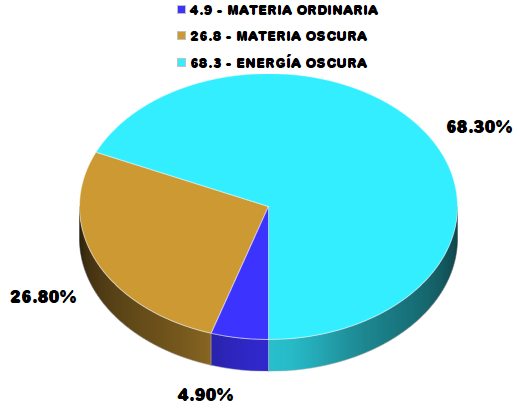
\includegraphics[width=0.49\textwidth]{Fisica_de_Particulas/imagenes/composicion0.png}
%\caption{Composición de la materia en el universo. Página de origen: %
%\url{https://wmap.gsfc.nasa.gov/media/121236/index.html}}
%\label{universo}
%\end{figure}





